%%This is a very basic article template.
%%There is just one section and two subsections.
%%This is a very basic article template.
%%There is just one section and two subsections.
\documentclass[a4paper,11pt,oneside,brazilian]{article}

\usepackage[utf8]{inputenx}
\usepackage[brazilian]{babel}
\usepackage{graphicx}
\usepackage{float}
\usepackage{textgreek}
\usepackage{mathtools}
\usepackage{enumerate}
\usepackage{xfrac}

\usepackage{multicol}

\usepackage{pgf,tikz}
\usepackage{pgfplots}
\usetikzlibrary{arrows}

\newcommand{\degre}{\ensuremath{^\circ}}
\newcommand{\bfig}{\begin{figure}[!h]\centering}
\newcommand{\efig}{\end{figure}}
\renewcommand{\thesection}{\Roman{section}}


\definecolor{zzttqq}{rgb}{0.6,0.2,0}
\definecolor{xdxdff}{rgb}{0.49,0.49,1}
\definecolor{qqqqff}{rgb}{0,0,1}
\definecolor{cqcqcq}{rgb}{0.75,0.75,0.75}
\definecolor{uuuuuu}{rgb}{0.27,0.27,0.27}
\definecolor{uququq}{rgb}{0.25,0.25,0.25}
\definecolor{qqwuqq}{rgb}{0.0,0.39215686274509803,0.0}
\definecolor{ffqqqq}{rgb}{1.0,0.0,0.0}
\definecolor{ffffff}{rgb}{1,1,1}

\pgfplotsset{compat=1.9}
\begin{document}

\title{Exercícios UERJ}
\author{Prof. Eduardo Elael}
\date{Lista UERJ 2ª fase - PVNC 2014}
\maketitle


\begin{flushright}
\emph{Data da realização:} nov/2014
\end{flushright}

\section{Matemática}
\begin{enumerate}[{R}1]
  
  \item A figura abaixo representa um triângulo equilátero, \(\overline{FN} =
  8, \overline{NG} =4\).
  Calcule \(\overline{HJ}\).
  
  \nopagebreak[4]
  \begin{figure}[H]
	\centering
	\begin{tikzpicture}[scale=0.8,line cap=round,line join=round,>=triangle
	45,x=1.0cm,y=1.0cm] \clip(9.680000000000003,-4.8) rectangle (24.52000000000001,8.820000000000002);
	\fill[color=zzttqq,fill=zzttqq,fill opacity=0.1] (11.0,-3.0) -- (23.0,-3.0) -- (17.000000000000004,7.392304845413266) -- cycle;
	\draw [shift={(19.0,-3.0)},color=qqwuqq,fill=qqwuqq,fill opacity=0.1] (0,0) -- (70.8933946491309:0.6000000000000003) arc (70.8933946491309:100.89339464913088:0.6000000000000003) -- cycle;
	\draw [color=zzttqq] (11.0,-3.0)-- (23.0,-3.0);
	\draw [color=zzttqq] (23.0,-3.0)-- (17.000000000000004,7.392304845413266);
	\draw [color=zzttqq] (17.000000000000004,7.392304845413266)-- (11.0,-3.0);
	\draw (19.0,-3.0)-- (20.5,1.3301270189221934);
	\draw (17.000000000000004,7.392304845413266)-- (19.0,-3.0);
	\begin{scriptsize}
	\draw [fill=qqqqff] (11.0,-3.0) circle (1.5pt);
	\draw[color=qqqqff] (10.580000000000004,-3.2999999999999994) node {$F$};
	\draw [fill=qqqqff] (23.0,-3.0) circle (1.5pt);
	\draw[color=qqqqff] (23.380000000000006,-3.4199999999999995) node {$G$};
	\draw [fill=uuuuuu] (17.000000000000004,7.392304845413266) circle (1.5pt);
	\draw[color=uuuuuu] (17.140000000000004,7.680000000000002) node {$H$};
	\draw [fill=qqqqff] (19.0,-3.0) circle (1.5pt);
	\draw[color=qqqqff] (19.000000000000007,-3.2999999999999994) node {$N$};
	\draw[color=qqwuqq] (19.100000000000005,-1.8199999999999994) node {$30\textrm{\degre}$};
	\draw [fill=uuuuuu] (20.5,1.3301270189221934) circle (1.5pt);
	\draw[color=uuuuuu] (20.640000000000008,1.6200000000000014) node {$J$};
	\end{scriptsize}
	\end{tikzpicture}
  \end{figure}
%\nopagebreak[4]
\pagebreak[4]
\item Uma pirâmide como a da figura abaixo possui todos os três ângulos
relativos ao vértice $A$ iguais a $60\degre$. Determine o seno do ângulo
$\hat{DBE}$


\begin{figure}[H]
\centering
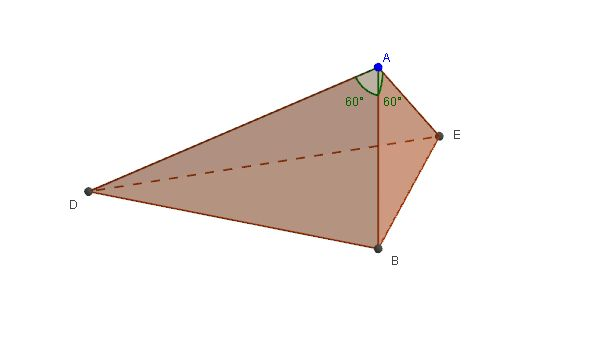
\includegraphics[width=1\columnwidth]{piramid.jpg}
\label{fig:cube}
\end{figure}


%\pagebreak[4]
\item Uma função quadrática $F(x)$ tem seu gráfico exibido abaixo:

\begin{figure}[H]
\centering
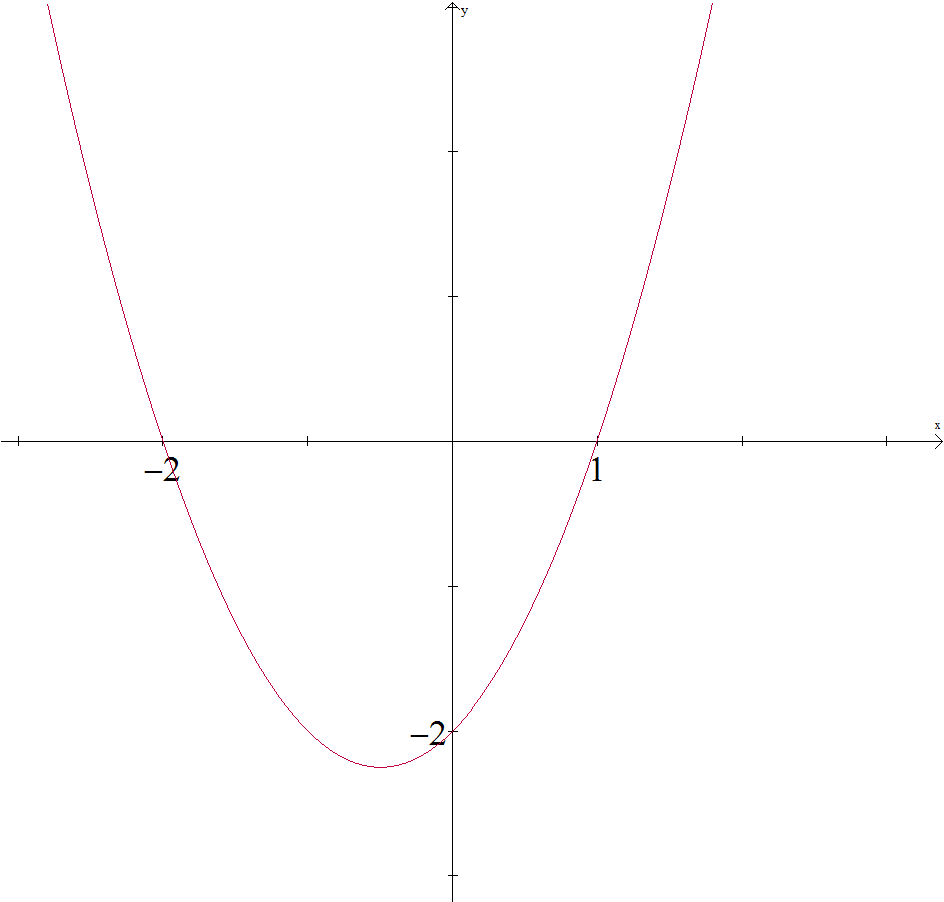
\includegraphics[width=0.5\columnwidth]{parabole.png}
\label{fig:cube}
\end{figure}
 

Essa função $F(x)$ é multiplicada por uma função polinomial $P(x)$ e resulta no
seguinte polinómio:

\[ x^4-x^3-2x^2+6x-4 \]

Entre as raízes de $P(x)$.


\nopagebreak[4]

\item Um míssil é lançado de um ponto $A$ fazendo um ângulo $\alpha$ com o
segmento $\overline{AC}$. Em $C$ se encontra um sistema de defesa que lançou
outro projetil em resposta, no mesmo instante, e foi capaz de interceptar o
míssil em um ponto $B$. Sabendo que tanto o míssil quanto o projetil de defesa
percorrem trajetórias retilíneas, e que a velocidade do míssil é 3 (três)
a do projetil. Calcule o seno do ângulo $\hat{BCA}$ que o projetil foi
lançado, em função do ângulo $\alpha$.

\begin{figure}[H]
\centering
\begin{tikzpicture}[scale=0.9,line cap=round,line join=round,>=triangle
45,x=1.0cm,y=1.0cm] \clip(2.96,-4.82) rectangle (15.9,-1.24);
\draw [shift={(4.,-4.)},color=qqwuqq,fill=qqwuqq,fill opacity=0.1] (0,0) -- (0.:1.5) arc (0.:11.2214642558:1.5) -- cycle;
\draw (4.,-4.)-- (15.,-4.);
\draw [->] (4.,-4.) -- (12.8900962031,-2.23625229476);
\draw [->] (15.,-4.) -- (12.8900962031,-2.23625229476);
\begin{scriptsize}
\draw [fill=qqqqff] (15.,-4.) circle (1.5pt);
\draw[color=qqqqff] (15.38,-4.24) node {$C$};
\draw [fill=qqqqff] (4.,-4.) circle (1.5pt);
\draw[color=qqqqff] (3.66,-4.06) node {$A$};
\draw [fill=qqqqff] (12.8900962031,-2.23625229476) circle (1.5pt);
\draw[color=qqqqff] (12.92,-1.76) node {$B$};
\draw[color=qqwuqq] (6.76,-3.68) node {$\alpha$};
\end{scriptsize}
\end{tikzpicture}
\end{figure}

\nopagebreak[4]
\item Para o mesmo sistema da questão anterior, agora é a apresentada a região
para a qual o projetil consegue interceptar o míssil, tendo o míssil 3 (três)
vezes a velocidade do projetil. Calcule o seno do ângulo $\alpha$ máximo,
para o qual o projetil ainda é capaz de atingir o míssil.

\item Sabendo que o polinômio abaixo possui raízes: $-2-i; -2+i; -0,1; 0,5; 5$,
onde $i$ é a unidade imaginária. Calcule as demais raízes desse polinômio: 
\[x^7 - 2,4 x^6 - 15,25 x^5 - 1,5 x^4 + 59x^3 + 28,4 x^2 - 22,75 x - 2,5 \]

\item Considere a seguinte matriz dependente do parâmtro $\theta$:

  \[ A(\theta) = 
	\begin{bmatrix}
	cos(\theta) & -sin(\theta)\\
	sin(\theta) & cos(\theta)\\
	\end{bmatrix}
  \]
  
  Definimos agora a matriz $B=A(12)*A(17)$. Calcule o valor numérico exato do
  determinante de $B$.

\end{enumerate}

\end{document}
